\documentclass[]{article}
\usepackage[utf8]{inputenc}
\usepackage{graphicx}
\usepackage{cancel}
\usepackage{emptypage}
\usepackage{subcaption}
\usepackage{hyperref}
\usepackage{url}
\usepackage{mathrsfs}
\usepackage{amsmath}
\usepackage{amsfonts}
\usepackage{ amssymb }
\usepackage{mathcomp}
\usepackage{gensymb}
\usepackage{tensor}
\usepackage{tcolorbox}
\usepackage{lmodern}
\usepackage{wasysym}
\usepackage{enumerate}
\setlength{\parindent}{2.0em}
\setlength{\parskip}{0.6em}
\renewcommand{\baselinestretch}{1.25}

\usepackage{geometry}
\geometry{
	a4paper,
	total={170mm,257mm},
	left=35mm,
	right=35mm,
	top=25mm,
}
%opening
\title{Recovery of DESI BGS redshift measurements using Machine Learning}
\author{Sergio Daivd Lobo Bolaño}

\begin{document}

\maketitle

\begin{abstract}
DESI (Dark Energy Spectroscopic Instrument) uses a simulated survey of mock galaxies to compare their redshifts with its -also simulated- redshift measurement. In this monograph we apply machine learning (ML) methods to the simulation data of DESI to recover the true redshift measurements of the Bright Galaxy Sample using observational variables as input, obtaining a $r^2 = 0.98$ using kernel and ensemble methods. 
\end{abstract}

\section{Introduction}
The redshift measurements of DESI present differences with respect to the true redshifts values of the mock galaxies used in simulations. It is necessary to correct these measurements so that the instrument can work properly when tested in the real world. One possible way is to use machine learning to recover the true redshift from the mock galaxies from observational variables as input. Therefore, this monograph has as main objective to recover the true redshifts of Bright Galaxies using observational variables from the simulated DESI measurements as an input to machine learning models, to improve the accuracy of DESI when used in the real world 

To accomplish this, first we pre-process the data and select the variables as input for the ML models, these variables are the fluxes from the different observation bands, which are the $g, r, z, WISE 1,$ and $WISE 2$ bands, as well as the redshift output of the instrument's pipeline. The true redshift from the mock galaxies is used as output. We train and test support vector regression (SVR) and kernel ridge regression (KRR) models using cross-validation and grid search, later we use an ensemble model of different KRRs. 
 
%\subsection{General Objective}
%\begin{itemize}
%	\item Recover the true redshifts of Bright Galaxies using observational variables from the simulated DESI measurements as an input to kernel methods of machine learning, to improve the accuracy of DESI when used in the real world
%\end{itemize}
\section{Methodology}
 First, we show a description of the data pre-processing, then the selection of computer parameters and finally, a description of the methodology for training and testing the models. Figure \ref{fig:generalmet} shows the general methodology for the project, each step will be treated below.  
\begin{figure}[ht!]
	\centering
	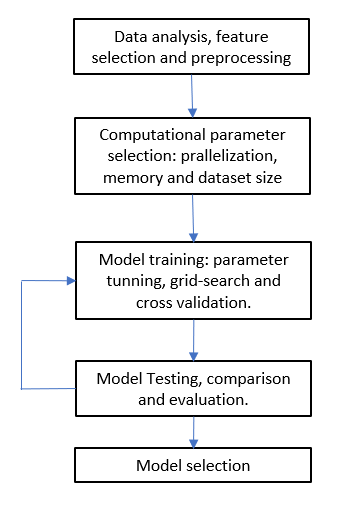
\includegraphics[width=0.4\linewidth]{TeX_files/Imagenes/general_met}
	\caption{General methodology for the project.}
	\label{fig:generalmet}
\end{figure}

The total dataset of size 889.336 was divided into training-test subsets of relative size 75 - 25. The training subset was used for training and selecting hyper-parameters by using grid search and cross validation. Figure \ref{fig:metho3} shows the data subgrouping.

During training, the development-evaluation stage was made on a even smaller subset inside the training set of size 100.000, due to computational resources. Therefore, to avoid sub-training the models we trained them in three different "sub-training" sets of size 100.000 each, and after that, we created an ensemble model with the combined responses of each one. In the Results section we explain this further.  

\begin{figure}[h!]
	\centering
	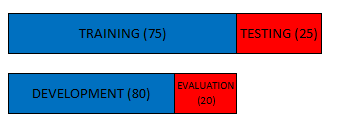
\includegraphics[width=0.6\linewidth]{TeX_files/Imagenes/metho_3}
	\caption{Division of the dataset in train and test. The train set is divided in development-evaluation subsets.}
	\label{fig:metho3}
\end{figure}

\section{Data Overview}

The true redshift (from the mock galaxies) and the target redshift (as measured by DESI) of BGS galaxies should in principle be equal, however, due to propagating error and misclassification in the data pipeline, the predicted redshift of the objects may have a deviation from its true value. Figure \ref{fig:bgs-z-truez} shows relation between the true redshift (TRUEZ) and the target redshift (TARZ). 
\begin{figure}[h!]
	\centering
	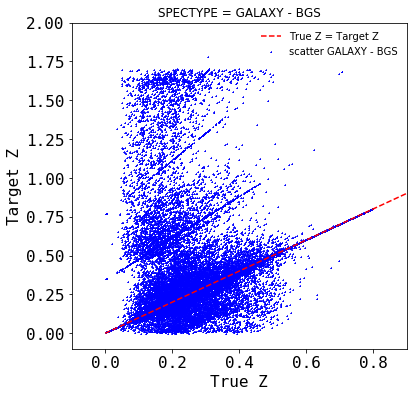
\includegraphics[width=0.6\linewidth]{TeX_files/Imagenes/BGS-z-truez}
	\caption{True and Target redsfhit relationship for BGS galaxies in the dataset. The red line indicates the line of calibration where the predicted redshift (target) is equal to the redshift of the galaxy (true) }
	\label{fig:bgs-z-truez}
\end{figure}

In order to plot the relation between TRUEZ, TARZ and other variables, we defined a new variable $\alpha$ as
\begin{equation}
\alpha = \frac{TRUEZ}{TARZ}.
\end{equation}
Therefore, $\alpha$ will take values of 1 when $TRUEZ = TARZ$ and other if their are different, the larger (or smaller) $alpha$, the larger the difference between the two redshifts. We plot in Figure \ref{fig:BGS-FLUX-ALPHA} the Flux G, R, Z, W1 and W2 to see if there was a pattern between this variables and $\alpha$. 
\begin{figure}[!htp]
	\centering
	\begin{subfigure}[t]{0.5\textwidth}
		\centering
		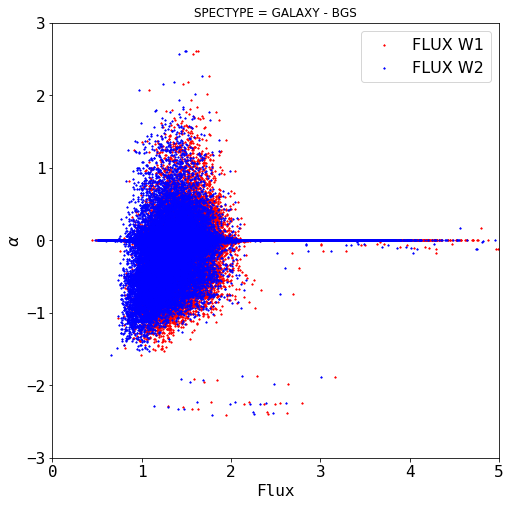
\includegraphics[height=3in]{TeX_files/Imagenes/BGS-FLUXW-ALPHA}
		\caption{}
	\end{subfigure}%
	\begin{subfigure}[t]{0.5\textwidth}
		\centering
		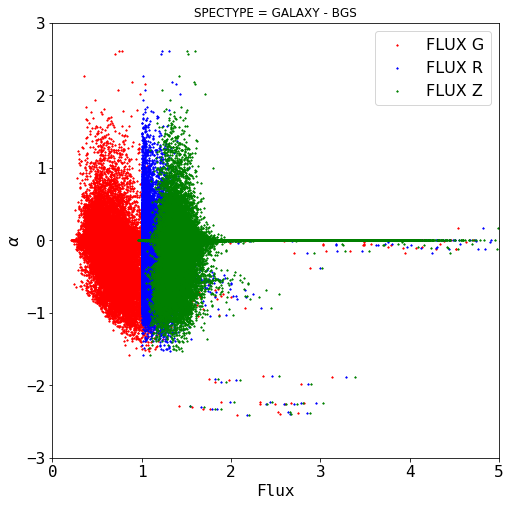
\includegraphics[height=3in]{TeX_files/Imagenes/BGS-FLUXRGZ-ALPHA}
		\caption{}
	\end{subfigure}
	\caption{Relation between fluxes, TRUEZ and TARZ. (a) $\alpha$ as a function of W1 and W2 fluxes. (b)$\alpha$ as a function of G, R and Z fluxes. $\log_{10}$ values presented.}
	\label{fig:BGS-FLUX-ALPHA}
\end{figure} 

From Figure \ref{fig:BGS-FLUX-ALPHA} we see that ther is a relation betwen the FLUXES variables and the redshifts encoded in $\alpha$, for this reason, we choose as input variables for the machine learning model: $\log_{10}(FLUX_G)$, $\log_{10}(FLUX_R),$ $\log_{10}(FLUX_Z),$  $\log_{10}(FLUX_{W1}),$  $\log_{10}(FLUX_{W2})$ and $TARZ$. For the predicted variable we chose $TRUEZ$, so our model takes in observational information \textit{and} DESI's predicted redshift to \textit{recover} the \textbf{true redshift} of the object. 

\section{Results}
The dataset was split in a training set (75\%) and a test set (25\%). We trained three SVR and three KRR models on random subsets of the training set of size 100.000 each due to memory and training time problems, this subset was also subdivided in an 80-20 development - evaluation datasets for the application of grid search and cross-validation. The three KRR outperformed the three SVR models, then the KRR were ensemble together to produce a single oputput as Figure \ref{fig:ensemblemodel} shows. The results of the three models on the training  development set is shown in Figure \ref{fig:krr-train} and \ref{fig:krr-test}.
  
\begin{figure}[h!]
	\centering
	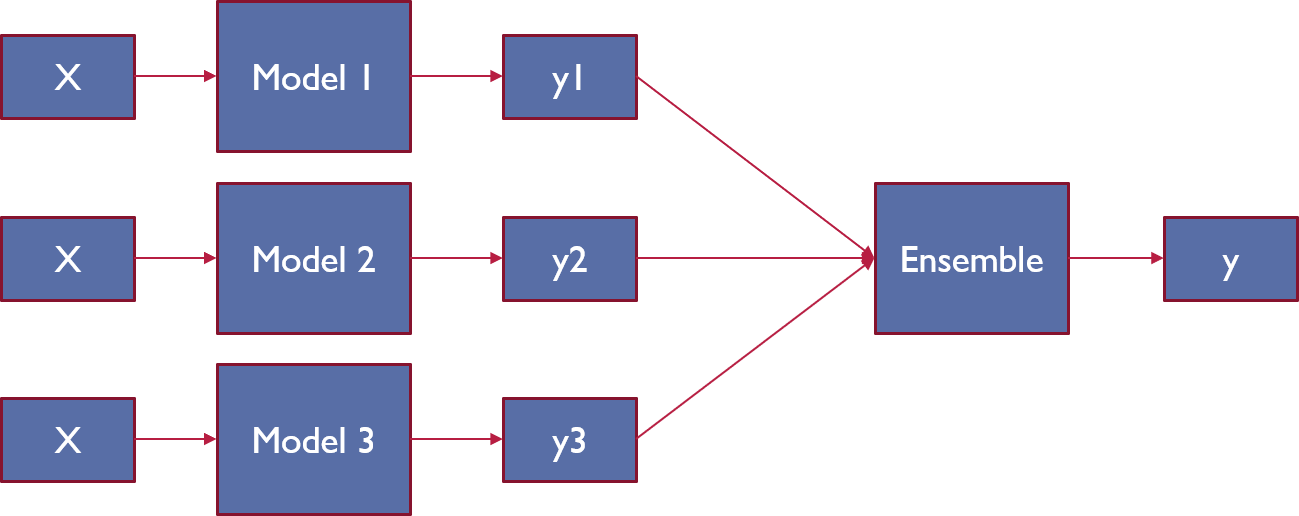
\includegraphics[width=0.8\linewidth]{TeX_files/Imagenes/ensemble_model}
	\caption{Graphic description of the ensemble model. It is formed based on the trained KRR models, each model previously trained on a random subset of size 100.000}
	\label{fig:ensemblemodel}
\end{figure}
\begin{figure}[th!]
	\centering
	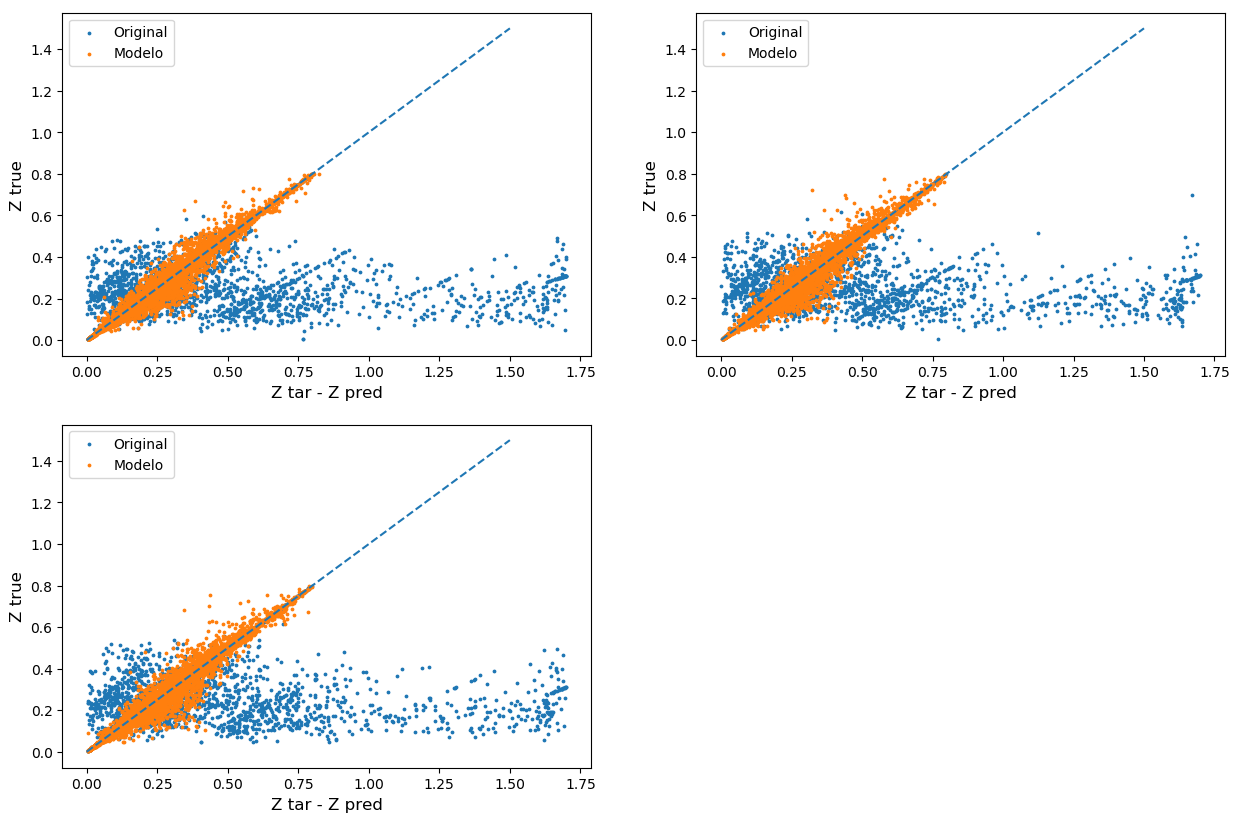
\includegraphics[width=1.0\linewidth]{TeX_files/Imagenes/krr-train}
	\caption{Results on the training set after training the KRR model.}
	\label{fig:krr-train}
\end{figure}
\begin{figure}[th!]
	\centering
	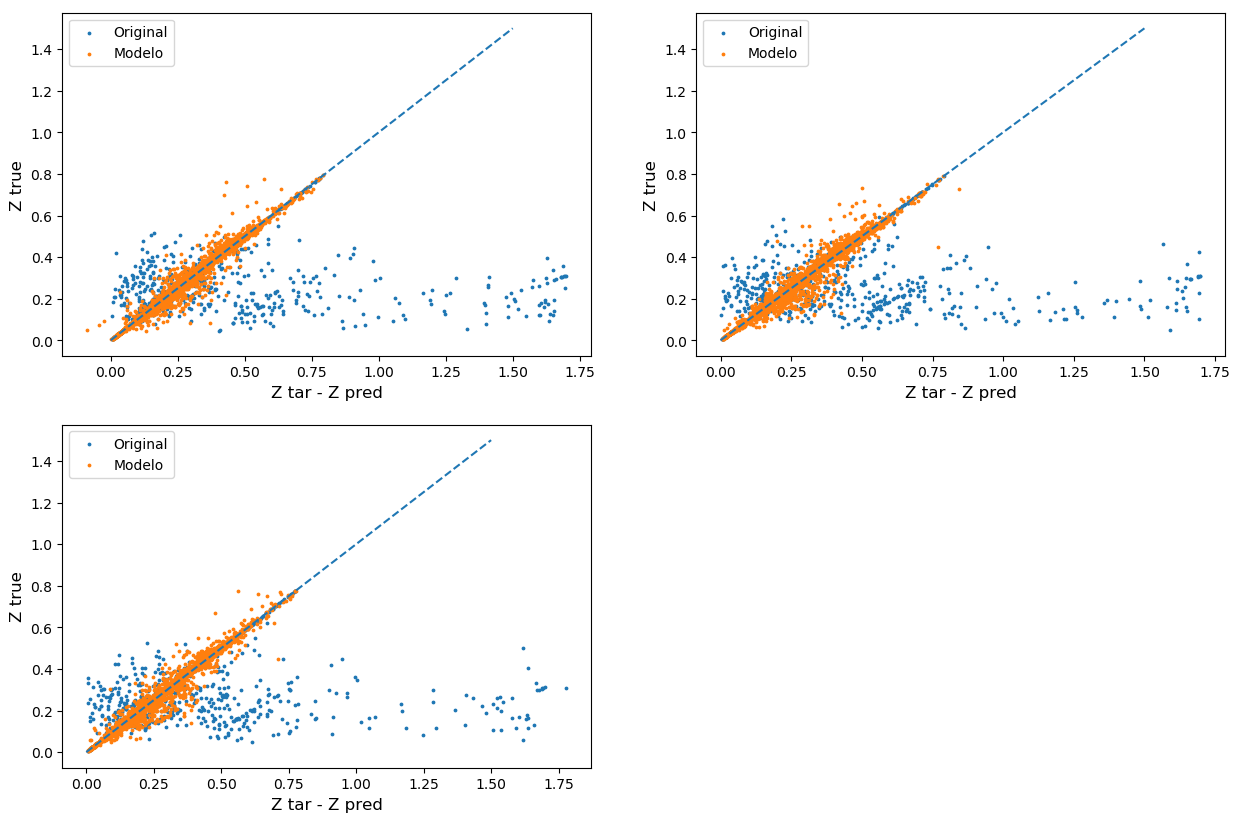
\includegraphics[width=1.0\linewidth]{TeX_files/Imagenes/krr-test}
	\caption{Results of each KRR model on the development set after training.}
	\label{fig:krr-test}
\end{figure}

Table \ref{table:test-result} shows the coefficient of determination, $r^2$  for each regression model on the testing(unseen) subset. The coefficient of determination estimated over $n_{samples}$ is defined as
\begin{equation}
	r^2 (y, \hat{y}) = 1 - \frac{\sum_{i = 0}^{n_{samples} - 1} \left(y_i - \hat{y_i}\right)^2}{\sum_{i = 0}^{n_{samples} - 1} \left(y_i - \bar{y_i}\right)^2},
\end{equation}
where $\hat{y_i}$ is the predicted value of the \textit{i}-th sample and $y_i$ is the corresponding true value.



\begin{table}[h!]
	\centering
	\begin{tabular}{|c|c|}
		\hline 
		Model & $r^2$ \\ 
		\hline 
		Model 1 & 0.958 \\ 
		\hline 
		Model 2 & 0.956 \\ 
		\hline 
		Model 3 & 0.962 \\ 
		\hline 
		Model avg & 0.962 \\ 
		\hline 
		Model max & 0.949 \\ 
		\hline 
		Model w & 0.983 \\ 
		\hline 
	\end{tabular} 
	\caption{Results on the \textbf{test} set for the three KRR model and the ensembles. Model w corresponds to training a linear model to find the best weight coefficients of each of the three models.}
	\label{table:test-result}
\end{table}

\section{Conclusions}
The object of this monograph was to apply machine learning (ML) methods to data coming from DESI end-to-end simulations to correct (or recover) true redshift of Bright Galaxies using observational variables as input. 

We found that the true redshift of the Bright Galaxy Sample (BGS) can be recovered using the variables FLUX\_G, FLUX\_R, FLUX\_Z, FLUX\_W1 and FLUX\_W2 as input to kernel methods. Using an ensemble model consisting of three KRRs (Kernel Ridge Regression) trained on subsamples of size 100.000, we were capable of approximate the DESI instrument redshift measurements to its true value up to a coefficient of determination $r^2 = 0.98$.  This model shows great potential to further enhancement, i.e. the fine-tuning of the model hyper-parameters, different classes of machine learning algorithms, as well as further use of ensemble methods with more than three "subtraining" sets in order to reduce bias.

The trained models did not work when tested in other classes of galaxies, probably because of the different distributions of fluxes. However, we infer that the same methodology could be used starting by training the models in the corresponding datasets. We expect that by doing so, the results of this work can be replicated and applied to all the classes in DESI. 
\end{document}
